\chapter{Review of Related Literature}
This section presents the reviewed literature from several readings of some research papers from the internet. The researcher synthesized the reading materials to emphasize insights relevant to the study. The organization of the reviewed materials consists of four sub-sections: Fish Classification and Identification, Object Detection Technologies, Fish Identification Using Machine Learning and Deep Learning, and YOLO Algorithm and Its Applications.
\section{Fish Classification and Identification}
Fish classification is a well-researched subject in the fields of information retrieval, pattern recognition, and picture segmentation. It has been used in innumerable fields, including information retrieval, target marketing, and recognition. Target marketing is only one of the many fields in which it has been used (Alsmadi and Almarashdeh, 2020). Traditional classifications are not only time-consuming and labor-intensive but they also are harmful, like a physical collection of fish samples by divers. 
A historical review of Computer Visions (CV) and Deep Learning using underwater cameras for fish classification and analyzing how their accuracy has evolved over the years, was conducted by Saleh et al (2022). The researchers first conducted a survey of the studies regarding fish classification in underwater habitats from 2003 to 2021, then an overview of the concepts of DL while synthesizing the studies. A total of 43 papers were reviewed, 26 of which are on classical computer vision methods and 17 on Deep Learning. Upon analyzing the papers, they found that publications on fish classification have been gradually increasing, specifically in 2016 when there were already few studies combining deep learning with computer vision, which was observed as the year with the highest increase of studies in fish classification with the highest value of accuracy. Furthermore, the researchers pointed out four challenges in fish classification which include the development of models that can generalize their learning and perform well on new unseen data samples, limited data sets available for general DL tasks, and in particular for marine visual processing tasks, lower image quality in underwater scenarios, and the gap between DL and ecology. Along with these, they proposed approaches to address these challenges. To monitor overfitting and develop a model that can generalize learning and perform well, there should be plotting and validation of the accuracy at each epoch during training. To address limited data sets, they highlighted several techniques applied to fish and marine habitats including, transfer learning, data augmentation, using hybrid features, weakly supervised learning, and active learning. Employing DL-based algorithms can enhance the quality of images underwater for better performance. To bridge the gap between DL and ecology, there is a need to develop and test general methods to estimate the absolute abundance of fish from very little data, along with developing general methods that can take advantage of the ecological knowledge and domain-specific data from a particular problem. Finally, they emphasized the importance of Deep Learning along with these techniques for providing a reliable means of classification and monitoring of fish habitats, and marine ecosystems. 
\section{Object Detection Technologies}
One of the most complicated and fundamental issues in computer vision is Object Detection, and for years it has been paid attention to. In the past 20 years, Object Detection can be regarded as the essence of computer vision history. The majority of the early algorithms for object detection were developed utilizing manually crafted features. In light of the insufficient efficacy of image representation during the early periods, individuals were compelled to develop intricate feature representations, alongside an array of optimization techniques to maximize the utilization of constrained computational resources (Zou et al., 2023). 
According to Soviany and Ionescu (2018), there are two types of deep learning techniques being used for target categorization and regression. On the one hand, we have single-stage detectors, exemplified by YOLO (You Only Look Once) and SSD (Single Shot MultiBox Detector), which conceptualize object detection as a straightforward regression challenge by processing an input image to derive class probabilities and bounding box coordinates. Although these models achieve comparatively lower accuracy rates, they exhibit significantly enhanced speed relative to their two-stage object detector counterparts. On the other hand, there exist two-stage detectors, like Faster R-CNN (Region-based Convolutional Neural Networks) or Mask R-CNN, which (i) create regions of interest in the first stage using a Region Proposal Network and (ii) send the region proposals down the pipeline for bounding-box regression and object classification. These models are usually slower, but they achieve the greatest accuracy rates.
Ren et al. (2015) introduced the Faster R-CNN object identification technique, which consists of four components: ROI pooling, region proposal network, feature extraction network, and a fully connected layer. Figure 1 depicts the entire detection procedure. The R-CNN and Fast R-CNN algorithms have been tweaked to create Faster R-CNN. The two differ in that the Faster R-CNN method generates candidate areas using the RPN rather than the computationally costly selective search approach. This approach significantly increases the detection speed of Faster R-CNN by calculating the characteristics of the entire image at once, eliminating the need for several computations (Tan et al., 2021).
Based on the study by Akshatha et al. (2022), SSD is a single-shot multi-box detector technique that detects multiple-scale items in a scene in a single step by using default anchor boxes and multi-scale characteristics. The anchor mechanism of Faster R-CNN and the end-to-end, one-step structure of the YOLO method, which performs object categorization and position regression immediately in the convolution stage, are the foundations of SSD, which was suggested by Liu et al. (2016).
YOLO, a novel method for object identification, was presented by Joseph et al. (2015). Classifiers are repurposed to carry out detection in earlier object detection operations. Rather, object detection is formulated as a regression problem to bounding boxes that are geographically separated and the class probabilities that go along with them. Bounding boxes and class probabilities are directly predicted from whole pictures in a single assessment by a single neural network. The detection pipeline may be directly optimized end-to-end on detection performance because it is a single network. The entire system simply requires a comparatively basic CNN structure to immediately finish the regression of target detection to forecast the candidate box's class and the bounding box's position. According to a recent study by Tan et al. (2021), object detection may be employed for real-time item identification and YOLO has an advantage in detection speed while maintaining a decent mean average accuracy.

\section{Fish Identification Using Machine Learning and Deep Learning}
Misidentification and variability in the accuracy of observers pose considerable challenges, as such errors can profoundly influence conservation and management initiatives. Neglecting to rectify possible species misidentification may culminate in erroneous evaluations of population status and distribution, ultimately leading to misguided conservation determinations (Austen et al., 2016).  Deep learning (DL), while still in its early stages within artificial intelligence, faces significant challenges in fish identification due to its reliance on extensive amounts of labeled data for training. This requirement has become a major obstacle, limiting progress in applying DL techniques to aquaculture (Yang et al., 2020). 
For numerous significant challenges, insufficient labeled data for training exists, and the generation of synthetic data is anticipated to be a pivotal methodology to alleviate this issue. It is imperative to guarantee that the images produced are specifically customized to the pertinent problem and to prevent the introduction of bias during the selection procedure. While it is a common challenge to have a limited dataset, retraining the part of the fish is another way to mitigate the problem, this approach is called transfer learning, where a system initially trained on a general or related task is adapted to the specific situation by retraining certain parts, typically the final layer of a neural network (Allken et al., 2018; Sharif Razavian et al., 2014; Yosinski et al., 2014). 
Wan et al (2021) proposed an identification algorithm for identifying freshwater fish species based on the improved ResNet50 Model. They took six types of freshwater fish including the bighead, bream, carp, crucian, grass carp, and silver carp as research objects. With these, they developed an image acquisition system and dataset combining laboratory and internet images. The improved model incorporated a fully connected layer, dropout, migration learning, CELU activation, Adam optimization, and cosine annealing. Results showed 96.94 percent accuracy (single validation), 100 percent (four-fold cross-validation, single-background,) and 96.20 percent (mixed-background), with an average detection time of 0.2345 seconds. The study revealed that the improved ResNet50 model presented a general structure and training, with a high accuracy rate under different backgrounds.
One of the most significant and notable challenges that are frequently encountered in the execution of this particular task pertains to the multifaceted nature of environmental changes that can drastically influence the results. Additionally, the issue of varied fish size presents considerable complexity, as it introduces a level of variability that complicates accurate identification and classification. Furthermore, feature variance emerges as a critical hurdle, as differences in morphological characteristics among species can lead to complications in analysis. Moreover, segmentation failure stands out as a prominent issue, characterized by the inability to accurately delineate and isolate individual fish from their surroundings in a given image. Lastly, the overarching problem of poor image quality must be addressed, as it significantly detracts from the clarity and usability of visual data, thereby impeding effective analysis and interpretation (Rachmatullah and Supriana, 2018).

\section{Mobile Applications for Fish Classification}
Pudaruth et al (2020) developed SuperFish, an innovative smartphone application for the identification of fish species that are commonly found in the lagoons and coastal areas, including estuaries and the outer reef zones of Mauritius consisting of 1520 images with 40 images for each of the 38 fish species. Among the data studied, 80 percent was used for training, 10 percent of which was for validation, and the remaining 10 percent was used for testing. The researchers utilized several classifiers such as kNN, Support Vector Machines, neural networks, decision trees, and random forests to identify what was the best-performing one. Firstly, All the images were converted into grayscale format. A Gaussian blur was then applied to remove the noise. To subtract the fish from the background, a thresholding operation was then performed on the images, enabling them to draw a contour around the fish from which several features were extracted. The researchers found that among the classifiers used, the kNN algorithm achieved the highest accuracy of 96 percent. Simultaneously, the TensorFlow framework, a model for recognition was created, resulting in an accuracy of 98 percent. The results implied the effectiveness of the software used in identifying fish species, driving them to increase the number of species to be studied, and to tackle challenging issues such as partial occlusions and pose variations through the use of more powerful deep learning architectures.
Similarly, Rossi et al (2020) proposed FishApp, a cloud-based infrastructure for fish species recognition. It is composed of a mobile application developed for the Android and the iOS mobile operating system enabling the user to capture pictures of a whole fish and submit them for remote analysis and a remote cloud-based processing system that implements a complex image processing pipeline and a neural network machine learning system able to analyze the obtained images and to perform classification into predefined fish classes namely, European Anchovies and the European Pilchards. The researchers then implemented a leave-one-out cross-validation (LOO-cv) model and an   ’in-field’ and ’ real-time’ fish to test the application’s species identification accuracy. The results revealed that  LOO-cv’s accuracy was 100 percent for the European Anchovies and the European Pilchards, implying that the application perfectly recognized both classes. 
The recent study by Liawatimena et al (2023) presented a method to detect fish and classify them on mobile devices by utilizing YOLO-v3 with RestNet as a backbone. The experiment focuses on training the model with only four types of fish. The results show that the YOLOv3-ResNet18 model produces 98.45 percent accuracy in training and 98.15 percent in evaluation, which concludes the suitability of the model for mobile devices that can sustain better precision and accuracy. Moreover, Dey et al (2023) proposed a mobile app for fish classification, FisHook, a mobile app that optimizes the MobileNetV2 model. The study article revealed outstanding accuracy in categorizing numerous marine species using data acquired via a mobile application. With a stated testing accuracy of 99.83 percent, this algorithm has the potential to play a critical role in marine conservation efforts, given the gains achieved over the status quo. In Bangladesh, Ataullha et al (2024) proposed the implementation of an automatic fish classification system namely, BanFish as a proactive initiative to promote familiarity with culturally significant fish in the country. It is considered the largest fish classification dataset designed for commonly available Bangladeshi fish. The researchers utilized 2,506 images spanning 18 distinct fish species, aimed to fill a critical void in preserving the diversity of indigenous fish. They employed a Vision Transformer with a transfer learning model to assess the dataset's quality, resulting in an overall accuracy of 83 percent. This implies that the proposed innovation serves as a valuable resource for fish classification offering a significant step toward preserving the rich tapestry of traditional fish species in Bangladesh. 

\section{YOLO Algorithm and Its Applications}

In recent years, advancements in object detection algorithms have transformed how visual classification tasks are performed in mobile and embedded systems. One of the most prominent applications of these advancements is in species identification—particularly fish classification. Priyankan and Fernando (2021) developed a mobile application based on a YOLO-based convolutional neural network (CNN) model to detect and identify the top-selling 16 Sri Lankan fish species. In addition to fish identification, the application offered informative features, such as nutritional content, pricing, and recipe suggestions. The study demonstrated that it is possible to build a deep learning-based classification model deployable on mobile platforms, though detection speed was influenced by internet connectivity, ranging from 3 to 20 seconds. In a similar context, Tharwat et al. (2018) emphasized the ecological importance of reliable fish species identification. They proposed a novel biometric-based classification method that involved three main phases. First, image features were extracted using Weber’s Local Descriptor (WLD) and color moments to capture both texture and color characteristics. Next, Linear Discriminant Analysis (LDA) was applied to reduce the feature dimensionality, and finally, an AdaBoost classifier was employed to identify species. The method yielded an impressive accuracy of 96.4\% and demonstrated robustness to image rotation and translation, confirming the potential of machine learning techniques in practical, real-world identification scenarios.

Expanding beyond fish classification, a growing body of literature has analyzed the architectural progression of object detection algorithms—particularly the YOLO (You Only Look Once) framework—which has evolved through multiple versions to balance detection accuracy and inference speed. Diwan et al. (2023) provided an in-depth review of single-stage object detectors, focusing on the innovations introduced across YOLO versions. YOLOv2 demonstrated improved multi-scale detection, while YOLOv3 featured a feature pyramid network for better representation of object hierarchies. YOLOv4, on the other hand, adopted a wide array of CNN optimization techniques aimed at further refining the trade-off between speed and precision. These architectural enhancements allowed YOLO models to outperform traditional two-stage detectors in many real-time applications. Chitraningrum et al. (2024) tested the efficacy of YOLOv5 and YOLOv8 in detecting diseased corn leaves. Their results showed that YOLOv8 significantly outperformed YOLOv5, achieving a mAP@50 of 0.965 compared to 0.727, thereby emphasizing the continuous improvement in detection precision within the YOLO family. Further reinforcing this trend, Sharma et al. (2024) conducted a comparative study involving YOLOv8, YOLOv9, YOLOv10, YOLOv11, and Faster R-CNN. The study focused on the detection of weed species including cocklebur, dandelion, Palmer amaranth, and lambsquarters under variable field conditions. A dataset comprising 2,348 annotated images was used to evaluate each model’s performance. The results revealed that YOLOv11 achieved the fastest inference time at just 13.5 milliseconds, while YOLOv9 attained the highest mAP@0.5 of 0.935. In contrast, Faster R-CNN lagged behind with the lowest accuracy and the slowest speed. This comparison highlighted YOLOv11’s effective balance between speed and accuracy, making it a leading choice for real-time applications in both agricultural and environmental monitoring domains.

Beyond agricultural use, recent research has extended YOLOv11's evaluation to more technically demanding applications, validating its capacity to perform well across a wide range of scenarios. Jegham et al. (2024) presented a benchmark evaluation of YOLOv11 against its earlier versions, focusing on model efficiency and precision. YOLOv11m was found to achieve a mean Average Precision (mAP50–95) of 0.795 while maintaining a compact model size of only 38.8 MB and achieving an average inference time of 2.4 milliseconds. These specifications position YOLOv11 as a strong candidate for deployment on mobile and embedded systems with limited resources. The model’s architectural improvements—specifically the inclusion of the C3k2 block and the Cross Stage Partial with Spatial Attention (C2PSA) module—enhanced its capacity to detect small, overlapping, and cluttered objects, an essential requirement for environments such as wet markets or densely populated aquatic image contexts. Ali and Zhang (2024) provided a comprehensive literature review on the YOLO framework’s progression from YOLOv1 to YOLOv11, documenting the technical innovations introduced in each iteration. The authors emphasized YOLOv11's improved robustness in low-light and occluded environments, as well as its real-time performance and ease of integration into embedded systems. These qualities extend the model’s usability far beyond typical RGB object detection. In particular, Bakirci and Bayraktar (2024) explored the application of YOLOv11 in detecting aircraft from Synthetic Aperture Radar (SAR) imagery. Their study assessed multiple YOLOv11 configurations—including nano, small, and medium models—and found that they delivered excellent detection accuracy for both large and distant aircraft targets, all while maintaining low computational overhead suitable for edge deployment on UAVs and drones. Similarly, Alif (2024) examined YOLOv11’s utility in the domain of intelligent transportation systems. The study used a complex dataset of vehicles—including cars, trucks, buses, motorcycles, and bicycles—and concluded that YOLOv11 outperformed YOLOv8 and YOLOv10, particularly in detecting small or occluded vehicles. It achieved higher values in precision, recall, and F1-score while retaining the speed needed for real-time performance in tasks like autonomous driving and traffic surveillance.

In summary, the literature presents consistent and growing evidence that YOLOv11 is among the most capable object detection models currently available for real-time and mobile-based applications. Its superior performance, reduced inference time, and architectural advancements make it an optimal choice for systems requiring high-speed and high-accuracy detection under variable and resource-constrained conditions. Whether applied to fish classification, weed detection, disease identification, aerial imaging, or vehicle recognition, YOLOv11 has proven its robustness, versatility, and suitability for deployment in real-world environments, making it a compelling backbone for next-generation mobile object detection systems.



\section{Summary}
Fish classification plays an important role not just in fishing and aquaculture industries but also in promoting cultural significance. These studies explored various aspects of deep learning and its application to classifying fish species. Techniques such as transfer learning, data augmentation, and mobile applications were utilized in these studies for fish classification. Moreover, some studies emphasized the use of YOLO (You Only Look Once) for fish detection and classification, with a focus on achieving high accuracy. Through these studies, the researchers gain insights into developing a fish identification system using the YOLO (You Only Look Once) v11 model, integrated into a mobile application for real-time fish classification, providing information on each identified species with improved accuracy, efficiency, and usability. 

\begin{landscape}
\begin{figure}[p]
    \centering
    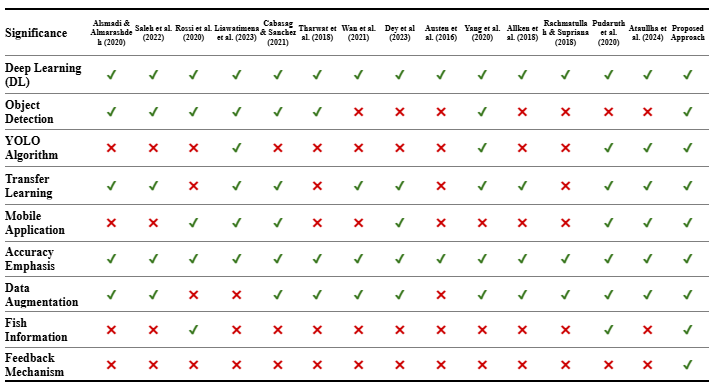
\includegraphics[height=0.80\textheight]{images/images/Summary_table_data.png}
    \caption{Table image: Comparison with Existing Studies for Fish Classification}
    \label{tab:comparison_existing_studies}
\end{figure}
\end{landscape}
